%!TEX root = ../template.tex
%%%%%%%%%%%%%%%%%%%%%%%%%%%%%%%%%%%%%%%%%%%%%%%%%%%%%%%%%%%%%%%%%%%%
%% chapter2.tex
%% NOVA thesis document file
%%
%% Chapter with the template manual
%%%%%%%%%%%%%%%%%%%%%%%%%%%%%%%%%%%%%%%%%%%%%%%%%%%%%%%%%%%%%%%%%%%%

\typeout{NT FILE GO-Babel.tex}

\chapter{GO-Babel}
\label{cha:GO-Babel}

The first contribution of this masters dissertation is an event-based framework called GO-Babel. This framework is a port in Golang \todo{citation} of Babel \todo{citation} with a few additions focused on fault detection and latency probing. Babel \todo{citation} itself is based on Yggdrasil \todo{citation}, which in turn is inspired on \todo{cite and discover paper of original event-based framework}.

The decision to build this framework arose from the need to use Babel for building the distributed protocols and the decision to use Golang during this dissertation (due to its primitives for building concurrent systems). Given that there was no implementation of Babel in Golang, and the current Babel implementation lacked needed features such as a fault detector and a latency measurement tool, we implemented a new version in Golang with these additions.

\section{Overview}

In summary, this framework has the following main objectives:

\begin{enumerate}

    \item Abstract the networking layer, providing \textbf{channels}, which are essentially an abstraction over TCP connections, providing callbacks whenever outbound or inbound connections are established or terminated and whenever messages or sent or received from the respective operating system buffers.

    \item Execute protocols in a single-threaded environment and provide abstractions for timers, request-reply patterns, notifications, and ease channel management.

    \item Provide a layer of abstraction over node latency probing and fault detection.

\end{enumerate}

\begin{figure}[htbp]
    \centering
    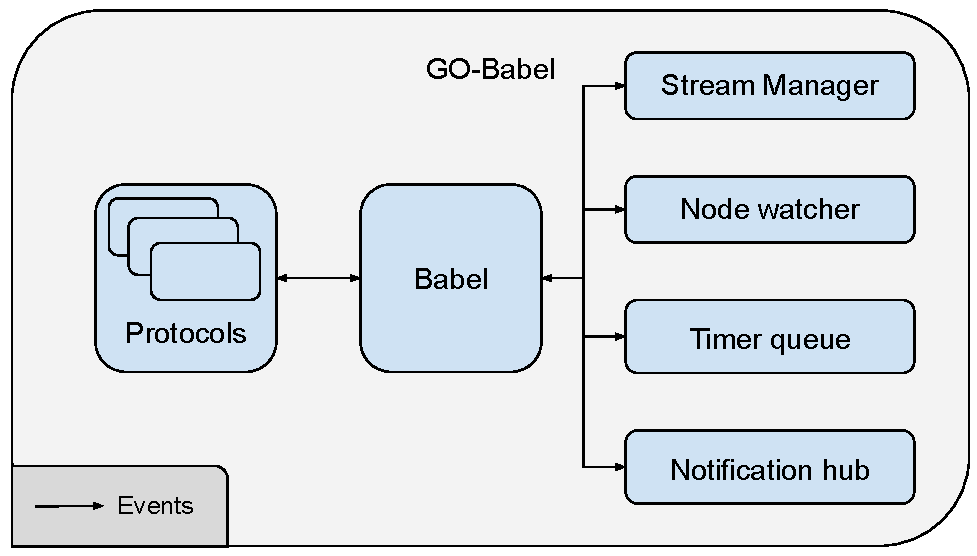
\includegraphics[width=\textwidth]{Chapters/Figures/Go-Babel-Overview.pdf}
    \caption{An overview of the architecture of GO-Babel}
    \label{fig:go-babel-overview}
\end{figure}

In the figure \ref{fig:go-babel-overview} we may observe a high-level overview of the architecture of this framework, composed of five main components which communicate via callbacks. We now summarize each components' roles in the framework:

\begin{enumerate}

    \item Babel is the component tasked with initializing the protocols and all the other components according to issued configurations. It also acts as a mediator between the protocols and the remaining components.

    \item The stream manager is responsible for handling incoming and outgoing connections, connecting to new peers, and sending messages. Whenever the state of any connection changes, the stream manager delivers events to protocols with the connection status (e.g. if the connection established, connection failure, message sent/received, connection terminated, among others). It also provides operations for sending messages in temporary connections (either using TCP or UDP).

    \item The timer queue allows the creation and cancellation of timers and manages the lifecycle of timers issued by the protocols, delivering events to protocols whenever timers reach their expiry time. The timer queue also allows creating periodic timers, which trigger at the set periodicity until cancelled.

    \item The notification hub is responsible for handling notifications and notification subscriptions, propagating issued notifications to registered subscribers (protocols).

    \item The node watcher allows for protocols to measure node latency and detect failures via a PHI-Accrual fault detector.

\end{enumerate}

As previously mentioned, the  Node Watcher is the only new addition to the framework, and consequently, it is the component explained in further detail. The remaining components of this framework were implemented similarly to Babel \todo{insert citation} and can found in \todo{cite}.

\section{Node Watcher} \label{sec:GO-Babel}

The node watcher is a component that, if registered, will listen for probes in a custom port (specified in the configurations) and send a reply with a copy of the contents back to the original senders. These probes are sent (usually) via UDP and carry a timestamp used by the original sender to calculate the round-trip time to the target node.

The motivation to build this component was a lack of tools to measure latency in the original design of Babel. If, for example, a protocol were to measure the latency to a node without an active connection, it would need to establish a new TCP connection and use it to send the probes. In this case, both the fault detector and latency detector logic are in the protocol, which is sub-optimal since the same logic would have to be replicated by any protocol that wishes to optimize its active connections using latency as a heuristic. Alternatively, if a protocol measures latencies in a separate module asynchronously (making the code reusable), this would break the single-threaded nature of the execution of protocols in Babel, and protocols would have to deal with race conditions of altering the state concurrently. Due to this, we believe that encapsulating this logic in an optional component and expose it in a Babel-compatible interface is the preferred option, which was the one used.

The main interface for the Node watcher is composed of two functions, ``watch'' and ``unwatch''. When a node is ``watched'', the node watcher starts sending probes to the target node according to the issued configuration settings and instantiates a PHI-accrual fault detector \todo{insert citation} together with a rolling-average latency calculator for that node. When the node receives replies with copies of sent probes, it updates the corresponding rolling average calculator and fault detector. Conversely, when a node is ``unwatched'', the node watcher stops issuing the probes and deletes the fault detector and latency calculator.


When a protocol issues a command to watch a node, if the ``watched'' node fails to reply within a time frame, the Node Watcher falls back to TCP. This fallback aims to overcome cases where the watched node may be dropping UDP packets due to a constraint in its infrastructure. If the watched node also does not accept the TCP connection, the node watcher sends a notification to the issuing protocol.


In order to prevent protocols from having to set timers to check the nodes' latency calculator or fault detector, the node watcher allows the possibility of registering ``observer'' functions (or conditions), which return a boolean value based on the current node information. The node watcher then executes these functions periodically, and if one returns true, a notification gets sent to the issuing protocol. In order to prevent protocols from getting overloaded with notifications when a condition returns ``true'', these may configure a grace period, which the node watcher will wait for until re-evaluating the condition.

\section{Conclusion}

We believe Go-Babel is a valuable contribution as it eases the implementation of self-improving protocols which employ latency as an optimization heuristic. In addition, it provides a secondary fault detector which may be employed together with the TCP connections. Lastly, as the implementation is in Golang \todo{cite}, it allows easier integration with a range of packages already implemented in the language. \todo{Sinto que esta secçao nao devia existir?}
